\documentclass[a4paper, 11pt]{article}
\usepackage{comment}
\usepackage{lipsum} 
\usepackage{fullpage} %cambiar margen
\usepackage[a4paper, total={7in, 10in}]{geometry}

\usepackage{amssymb,amsthm} 
\usepackage{amsmath}
\newtheorem{theorem}{Theorem}
\newtheorem{corollary}{Corollary}
\usepackage{graphicx}
\usepackage{tikz}
\usetikzlibrary{arrows}
\usepackage{verbatim}
%\usepackage[numbered]{mcode}
\usepackage{float}
\usepackage{tikz}
\usetikzlibrary{shapes,arrows}
\usetikzlibrary{arrows,calc,positioning}
\usepackage{mathpazo} %tipo de letra 
\usepackage[utf8]{inputenc} %codificación
\usepackage[T1]{fontenc} %digitación de tildes y ñ
\usepackage[spanish]{babel} %paquete de soporte español

\tikzset{
	block/.style = {draw, rectangle,
		minimum height=1cm,
		minimum width=1.5cm},
	input/.style = {coordinate,node distance=1cm},
	output/.style = {coordinate,node distance=4cm},
	arrow/.style={draw, -latex,node distance=2cm},
	pinstyle/.style = {pin edge={latex-, black,node distance=2cm}},
	sum/.style = {draw, circle, node distance=1cm},
}
\usepackage{xcolor}
\usepackage{mdframed}
\usepackage[shortlabels]{enumitem}
\usepackage{indentfirst}
\usepackage{hyperref}

\usepackage{listings}
\lstset{literate=
  {á}{{\'a}}1
  {é}{{\'e}}1
  {í}{{\'i}}1
  {ó}{{\'o}}1
  {ú}{{\'u}}1
  {Á}{{\'A}}1
  {É}{{\'E}}1
  {Í}{{\'I}}1
  {Ó}{{\'O}}1
  {Ú}{{\'U}}1
  {ñ}{{\~n}}1
  {ü}{{\"u}}1
  {Ü}{{\"U}}1
}

\lstdefinestyle{customc}{
  belowcaptionskip=1\baselineskip,
  breaklines=true,
  frame=L,
  xleftmargin=\parindent,
  language=Python,
  showstringspaces=false,
  basicstyle=\footnotesize\ttfamily,
  keywordstyle=\bfseries\color{green!40!black},
  commentstyle=\itshape\color{purple!40!black},
  identifierstyle=\color{blue},
  stringstyle=\color{orange},
}

\lstdefinestyle{customasm}{
  belowcaptionskip=1\baselineskip,
  frame=L,
  xleftmargin=\parindent,
  language=[x86masm]Assembler,
  basicstyle=\footnotesize\ttfamily,
  commentstyle=\itshape\color{purple!40!black},
}

\lstset{escapechar=@,style=customc}



\renewcommand{\thesubsection}{\thesection.\alph{subsection}}

\newenvironment{problem}[2][Ejercicio]
{ \begin{mdframed}[backgroundcolor= red!50] \textbf{#1 #2} \\}
	{  \end{mdframed}}

% Define solution environment
\newenvironment{solution}
{\textcolor{blue}{\textbf{\textit{Solución:\\\noindent}}}}


\renewcommand{\qed}{\quad\qedsymbol}

% \\	
\begin{document}
	\noindent
	%%%%%%%%%%%%%%%%%%%%%%%%%%%%%%%%%%%%
	
	\begin{minipage}[b][1.2cm][t]{0.8\textwidth}
		\large\textbf{César Isaí García Cornejo} \hfill \textbf{Tarea 1}  \\
		cesar.cornejo@cimat.mx \hfill \\
		\normalsize Estadística Bayesiana \hfill Semestre 4\\
	\end{minipage}
	
	\hspace{14.4cm}
	\begin{minipage}[b][0.03cm][t]{0.12\linewidth}
		
		\vspace{-2.2cm}
		%%%La Ruta dependerá de donde este alojado el main y la imagen
		
\includegraphics[scale=0.3]{Figures/EscudoCimat.png}
	\end{minipage}
	
	\noindent\rule{7in}{2.8pt}
	
	%%%%%%%%%%%%%%%%%%%%%
	%%%%%%%%%%%%%%%%%%%%%%%%%%%%%%%%%%%%%%%%%%%%%%%%%%%%%%%%%%%%%%%%%%%%%%%%%%%%%%%%%%%%%%%%%%%%%%%%%%%%%%%%%%%%%%%%%%%
	% Problem 1
	%%%%%%%%%%%%%%%%%%%%%%%%%%%%%%%%%%%%%%%%%%%%%%%%%%%%%%%%%%%%%%%%%%%%%%%%%%%%%%%%%%%%%%%%%%%%%%%%%%%%%%%%%%%%%%%%%%%%%%%%%%%%%%%%%%%%%%%%
	\setlength{\parskip}{\medskipamount}
	\setlength{\parindent}{0pt}
%/////////// Ejercicio 1 /////////////////
\begin{problem}{1} 
    Sea $X_i \sim Bi(k,P)$ cond. independientes $i = 1,2,...,n$, pero ambos $k$ (número de ensayos) y $p$ son desconocidos. ¿Cómo haría inferencia bayesiana en este caso? Ejemplo: $k$ individuos de cierta especie de mamífero, con la misma probabilidad $p$ de ser vistos, son muestreados de manera independiente. Los datos son los siguientes: 4 3 1 6 6 6 5 5 5 1 $(n=10)$. ¿ Qué puede decir sobre el total $k$ de individuos?
\end{problem}

\begin{solution} 
    Tenemos que la verosimilitud de los datos es
    \begin{align*}
        f(x^n|k,p) &= \prod_{i= 1}^{n} \left(\binom{k}{x_i}p^{x_i}(1-p)^{k-x_i}\right) \\
        &= \left(\prod_{i= 1}^{n} \binom{k}{x_i}\right) p^{\sum{x_i}}(1-p)^{kn - \sum{x_i}}
    \end{align*}
    Proponiendo las distribuciones a priori de los parámetros como
    \begin{align*}
        \pi(p) = \frac{\Gamma(\alpha + \beta)}{\Gamma(\alpha)\Gamma(\beta)}p^{\alpha -1 }(1-p)^{\beta-1},\\
        \pi(k) = \mathbb{1}_{\{X_{(n)}, X_{(n+1)},\cdots\}}(k)
    \end{align*}
    Notemos que la distribución a priori para $p$ es una beta y la distribución para $k$ es una priori impropia cuyo dominio son los naturales mayores o iguales que la estadística de orden superior $X_{(n)}$.

    La posterior conjunta dada por el Teorema de Bayes es
    \begin{align*}
        \pi(k,p|x^n) &\propto \left(\prod_{i= 1}^{n} \binom{k}{x_i}\right) p^{\sum{x_i}}(1-p)^{kn - \sum{x_i}}\frac{\Gamma(\alpha + \beta)}{\Gamma(\alpha)\Gamma(\beta)}p^{\alpha -1 }(1-p)^{\beta-1}\\
        &\propto \left(\prod_{i= 1}^{n} \binom{k}{x_i}\right) p^{\sum{x_i}+\alpha -1}(1-p)^{kn - \sum{x_i}+\beta -1}
    \end{align*}
    Podemos obtener la distribución marginal (salvo una constante) integrando respecto a $p$. Así
    \begin{align*}
        \pi(k|x^n) \propto \left(\prod_{i= 1}^{n} \binom{k}{x_i}\right)\int_{0}^{1} p^{\sum{x_i} + \alpha -1 }(1-p)^{kn - \sum{x_i} + \beta -1} dp 
    \end{align*} 
    De la normalización de la distribución beta sabemos que
    \begin{align*}
        \frac{\Gamma(kn + \alpha + \beta)}{\Gamma(\sum{x_i})\Gamma(kn - \sum{x_i}+\beta)}\int_{0}^{1} p^{\sum{x_i}+\alpha -1}(1-p)^{kn - \sum{x_i}+\beta -1} dp = 1
    \end{align*}
    Por tanto, la marginal tiene la siguiente forma funcional
    \begin{align*}
        \pi(k|x^n) &\propto \left(\prod_{i= 1}^{n} \binom{k}{x_i}\right)\frac{\Gamma(\sum{x_i})\Gamma(kn - \sum{x_i}+\beta)}{\Gamma(kn + \alpha + \beta)}\\
        &\propto \frac{\left(k!\right) ^n}{\prod_{i=1}^{n}(\left(x_i!(k-x_i)!\right) )} \frac{\left(kn-\sum{x_i}+\beta-1 \right)!}{(kn + \alpha + \beta-1)!}\\
        &\propto \frac{\left(k!\right) ^n}{\prod_{i=1}^{n}(k-x_i)!}\frac{\left(kn-\sum{x_i}+\beta-1 \right)!}{(kn + \alpha + \beta-1)!}
    \end{align*}

    Podemos calcular la distribución posterior para varios valores
    de $k$, 

    \begin{figure}[H] 
        \centering 
        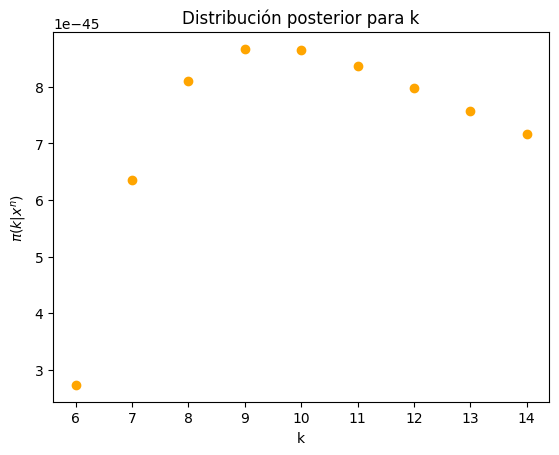
\includegraphics[width = 12 cm]{Figures/dist_especies1.png} 
        \caption{Distribución posterior de $k$ para $k$ entre 6 y 14.}
        \label{Fig. 01}
    \end{figure} 
    
    \begin{figure}[H] 
        \centering 
        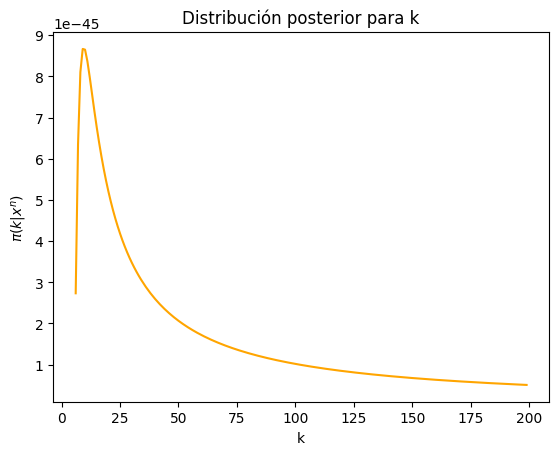
\includegraphics[width = 12 cm]{Figures/dist_especies.png} 
        \caption{Distribución posterior de $k$ para $k$ entre 6 y 200.}
        \label{Fig. 02}
    \end{figure} 

    Vemos que un buen estimador para $k$ es la moda de la distribución, que es el máximo de la posterior. Dicho valor es $k=9$ lo que nos da cierto grado de conocimiento acerca de la cantidad de población total.





\end{solution}




% \begin{problem}{2}
%     Partiendo del problema 1 suponga que ahora se plantea decidir el tamaño de muestra $n$, siendo que cada muestra nos cuesta $w $ pesos.
% \end{problem}

\begin{problem}{3}       
    Supón que con una probabilidad de 1/10  una señal está presente en cierto sistema en un momento dado y que con una probabilidad 9/10 la señal no está presente. Una medición hecha en el sistema cuando la señal está presente tiene una distribución Normal con media 50 y varianza 1 y una medición cuando la señal no stá presente tiene una distribución Normal con media 52 y varianza 1.
    \begin{enumerate}
        \item Supón que una medición $X$ hecha en el sistema en un momento dado es igual a $x$. Muestre que la probabilidad posterior de que la señal esté en el sistema es mayor de que no esté, dado $X = x$, si $x < 51 - \text{0.5} \log 9$.
        \item Dado que $X = 50$, demuestre que la esperanza predictiva de una nueva medición $Y$, independiente de la anterior, es aproximadamente \text{51.0932} .
    \end{enumerate}
\end{problem}


\begin{solution} 
    \begin{enumerate}
        \item 
        Consideremos el evento hay señal como S, al evento no hay señal como NS. Luego $\mathbb{P}\left (S \right ) = 1/10$ y $\mathbb{P}\left (NS \right ) = 9/10$. Además
        \begin{align*}
            S \Rightarrow X \sim N(50,1)\\
        NS \Rightarrow X \sim N(52,1)
        \end{align*}
        Calculemos las probabilidades (densidades) posteriores. Del Teorema de Bayes
        \begin{align}
            \mathbb{P}\left (S|X = x \right ) &= \frac{\mathbb{P}\left (X =x|S \right )\mathbb{P}\left (S \right )} {\mathbb{P}\left (X = x \right )}, \nonumber \\
            &= \frac{\mathbb{P}\left (X=x|S \right )\mathbb{P}\left (S \right )}{\mathbb{P}\left (X=x |S \right ) \mathbb{P}\left (S \right )+ \mathbb{P}\left (X = x|NS \right )\mathbb{P}\left (NS \right )} \nonumber \\
            &= \frac{\frac{1}{\sqrt{2\pi}}\exp{\left(-\frac{(x-50)^2}{2}\right)} \cdot \frac{1}{10} }{\frac{1}{\sqrt{2\pi}}\exp{\left(-\frac{(x-50)^2}{2}\right)} \cdot \frac{1}{10} + \frac{1}{\sqrt{2\pi}}\exp{\left(-\frac{(x-52)^2}{2}\right)} \cdot \frac{9}{10}}\nonumber\\
            &= \frac{\exp{\left(-\frac{(x-50)^2}{2}\right)}}{\exp{\left(-\frac{(x-50)^2}{2}\right)}  + 9\exp{\left(-\frac{(x-52)^2}{2}\right)} }
            \label{3.01}
        \end{align}

        De forma análoga calculamos la otra probabilidad. Sin embargo es más simple notando que 
        \begin{align*}
            \mathbb{P}\left (S|X = x \right ) +\mathbb{P}\left (NS|X = x \right ) = 1.
        \end{align*}
        Luego,
        \begin{align}
            \mathbb{P}\left (NS|X = x \right ) = \frac{9\exp{\left(-\frac{(x-52)^2}{2}\right)}}{\exp{\left(-\frac{(x-50)^2}{2}\right)}  + 9\exp{\left(-\frac{(x-52)^2}{2}\right)} }
            \label{3.02}
        \end{align}
        
        Busquemos que condiciones es necesaria tal que satisface
        \begin{align}
            \mathbb{P}\left (S|X = x \right ) > \mathbb{P}\left (NS|X = x \right )
            \label{3.03}
        \end{align}
        sustituyendo las ecuaciones (\ref{3.01}) y (\ref{3.02}) en (\ref{3.03}) tenemos
        \begin{align}
            \exp{\left(-\frac{(x-50)^2}{2}\right) } &> 9\exp{\left(-\frac{(x-52)^2}{2}\right) }\nonumber\\
            -\frac{(x-50)^2}{2} &> \log{9} - \frac{(x-52)^2}{2}\nonumber\\
            \frac{(x-52)^2}{2}-\frac{(x-50)^2}{2} &> \log{9} \nonumber\\
            -4x + 204 &> 2\log{9}\\
            x &< 51 - \frac{1}{2}\log{9}
            \label{3.04}
        \end{align}
        Así, la condición (\ref{3.04}) es suficiente para satisfacer (\ref{3.03}), lo que concluye la demostración.
        
        \item 
        Sea $Y$ la observación independiente posterior a $X$. Para calcular la esperanza predictiva, calculamos primero el valor de la distribución predictiva. Requerimos
        \begin{align}
            f(Y|X) &= \int f(Y|X,\theta)\pi(\theta|X) d\theta \nonumber\\
            &= 
        \end{align}
        En nuestro caso tenemos que la distribución posterior del parámetro es discreta ya que es la distribución de señal presente o señal ausente. De está forma se reduce a calcular
        \begin{align}
            f(Y|X) &= f(Y|S) \pi(S|X) + f(Y|NS) \pi(NS|X)\nonumber \\
            &= \frac{1}{\sqrt{2\pi}}\exp{\left(-\frac{(y-50)^2}{2}\right) } \cdot \pi(S|X) +\frac{1}{\sqrt{2\pi}}\exp{\left(-\frac{(y-52)^2}{2}\right) } \cdot \pi(NS|X)
        \end{align}
        Observemos que $\pi(S|x) = \mathbb{P}\left (S|X = x \right )$ y $\pi(NS|x) = \mathbb{P}\left (NS|X = x \right )$. 

        La esperanza predictiva es entonces una suma ponderada por las probabilidades posteriores. De esta forma
        \begin{align}
            \mathbb{E}\left [Y|X\right ] &= 50  \pi(S|X) + 52  \pi(NS|X) \nonumber\\
            &= 50\cdot \text{0.4508} + 52 \cdot \text{0.5491}\nonumber \\
            &= \text{51.0982}.
        \end{align}
        lo que concluye la cuenta.

    
    
\end{enumerate}


\end{solution}

\newpage

\begin{problem}{4} 
    A scientific journal, in a n attempt to maintain experimental standards, insists that all reported statistical results have (classical) error probability of $\alpha_0$ ( or better). To considere a very simple model of this situation, assume that all statistical tests conducted are of the form $ H_0: \theta = \theta_0$ versus $H_1: \theta = \theta_1$ , where $\theta_0$ represents the standard and $\theta_1$ the new proposal. Experimental results are reported in the journal only if the new proposal. Experimental results are reported in the journal only if the new proposal is verified with an error probability of $ \alpha \leq \alpha_0.$ (Nota that $\alpha = \mathbb{P}\left (\text{aceepting $H_1$} \right ))$. Let $\beta$ denote the power of the test (i.e., $\beta = \mathbb{P}_{\theta_1}\left ( \text{accepting } H_1 \right )$). Assume further that $\alpha$ and $\beta$ are fixed for all experiments conducted, with $\alpha$ being the specified value $\alpha_0$. Let $\pi_0$ denote the proportion of all experiments conducted in which $\theta_0$ is correct, and $\pi_1$ denote the proportion of experiments in which $ \theta_1$ is correct. 
    \begin{enumerate}
        \item Show that the proportion of articles published in the journal tha have correct results (i.e., \\
        $\mathbb{P}\left (\theta = \theta_1 | \text{the test accepts $H_1$}\right ))$ is $\pi_1 \beta /[\alpha_0+ \pi_1(\beta-\alpha_0)]$. (Note that many people naively believe that the journal in guaranteeing a proportion of $(1- \alpha_0)$ of correct articles.)
        \item Show that the proportion of correct published results is never less than $\pi_1$. (Note that $\beta \geq \alpha$ for reasonable tests.)
    \end{enumerate}
\end{problem}

\begin{solution} 
    \begin{enumerate}
        \item Observemos previamente que las proporciones de artículos asociados a $\theta_0$ mas las proporciones de artículos asociados a $\theta_1$ es uno, es decir, $\pi_0 + \pi_1 = 1$. Luego, del teorema de Bayes y la cantidad de interés se sigue
        \begin{align*}
            \mathbb{P}\left (\theta = \theta_1 |\text{test } H_1 \right ) = \frac{\mathbb{P}\left (\text{test } H_1| \theta = \theta_1 \right ) \mathbb{P}\left (\theta = \theta_1 \right )}{\mathbb{P}\left (\text{test } H_1 \right )}
        \end{align*} 
        De la ley de probabilidad total tenemos
        \begin{align*}
            \mathbb{P}\left (\theta = \theta_1 |\text{test } H_1 \right ) = \frac{\mathbb{P}\left (\text{test } H_1| \theta = \theta_1 \right ) \mathbb{P}\left (\theta = \theta_1 \right )}{\mathbb{P}\left (\text{test } H_1|\theta = \theta_1 \right )\mathbb{P}\left (\theta = \theta_1 \right ) + \mathbb{P}\left (\text{test } H_1|\theta = \theta_0 \right )\mathbb{P}\left (\theta = \theta_0 \right )}
        \end{align*}
        Recordemos que la probabilidad de rechazar $H_0$ dado que el parámetro es $\theta_1$ es la potencia. Entonces $\mathbb{P}\left (\text{test } H_1| \theta = \theta_1 \right ) = \beta$. Así, con la notación establecida
        \begin{align*}
            \mathbb{P}\left (\theta = \theta_1 |\text{test } H_1 \right ) &= \frac{\beta \pi_1}{ \beta \pi_1 + \alpha \pi_0}\\
            &= \frac{\beta \pi_1}{\beta\pi_1 + \alpha (1-\pi_1)}\\
            &= \frac{\beta \pi_1}{(\beta - \alpha)\pi_1 + \alpha}
        \end{align*}
        obteniendo la expresión esperada.
        
        \item Tomemos primero el caso $\alpha = \beta$. Entonces la probabilidad de interés es
        \begin{align*}
            \mathbb{P}\left (\theta = \theta_1 |\text{test } H_1 \right ) = \frac{\beta \pi_1}{0\pi_1 + \alpha} = \pi_1
        \end{align*}
        Para el caso $\beta > \alpha$ el denominador tenemos que $\beta > \beta - \alpha  $ con $\alpha$ positivo, luego como $\pi_1 \leq 1$ se sigue que $(\beta -\alpha)\pi_1 + \alpha <\beta \pi_1$ lo que concluye que el cociente tiene que ser mayor que $\pi_1$.
    \end{enumerate}
        






\end{solution}

\begin{problem}{5} 
    Suppose that $\mathbf{X} = (X_1, ..., X_n)$ is a sample from a $\mathcal{N}\mathcal{B}(m,\theta)$ distribution, and that $\theta $ has a $Beta(\alpha,\beta)$ prior distribution. Show that the posterior distribution of $\theta$ given $\mathbf{x}$ is $Beta(\alpha + mn, (\sum_{i=1}^{n}x_i)+ \beta)$.
\end{problem}


\begin{solution} 
  Recordemos la función de (masa de) probabilidad de la distribución binomial negativa. Para $X \in \{0,1,...\}$
  \begin{align*}
    f(x|\theta) = \frac{\Gamma(m+x)}{\Gamma(x+1)\Gamma(m)}\theta^m(1-\theta)^x
  \end{align*}
  Por tanto la verosimilitud de las observaciones se representa con la siguiente distribución conjunta
  \begin{align*}
    \mathcal{L}(\theta) &= f(x^n|\theta) \\&= \prod_{i = 1}^{n} \frac{\Gamma(m+X_i)}{\Gamma(X_i+1)\Gamma(m)}\theta^m(1-\theta)^{X_i}\\
    &= \left(\prod_{i = 1}^{n} \frac{\Gamma(m+X_i)}{\Gamma(X_i+1)\Gamma(m)}\right) \theta^{mn}(1-\theta)^{\sum_{i = 1}^{n}X_i} 
  \end{align*}
  Como la distribución a priori es:
  \begin{align*}
    \pi(\theta) = \frac{\Gamma(\alpha + \beta)}{\Gamma(\alpha)\Gamma(\beta)} \theta^{\alpha -1} (1- \theta)^{\beta -1}
  \end{align*}
  Entonces la distribución posterior sigue que
  \begin{align*}
    \pi(\theta|x^n) \propto \left(\prod_{i = 1}^{n} \frac{\Gamma(m+X_i)}{\Gamma(X_i+1)\Gamma(m)}\right) \theta^{mn}(1-\theta)^{\sum_{i = 1}^{n}X_i} \frac{\Gamma(\alpha + \beta)}{\Gamma(\alpha)\Gamma(\beta)} \theta^{\alpha -1} (1- \theta)^{\beta -1}
  \end{align*}
  simplificando
  \begin{align*}
    \pi(\theta|x^n) \propto \theta^{nm+\alpha -1} (1- \theta)^{\sum X_i + \beta -1 }
  \end{align*}
  que es el kernel de la distribución beta. Así
  \begin{align*}
    \theta|X^n \sim Beta(nm + \alpha, \sum X_i + \beta)
  \end{align*}
  lo que concluye el ejercicio.

\end{solution}

% \begin{thebibliography}{9}

%     \bibitem{Casella}
%     Robert, C. P., Casella, G., and Casella, G. (1999). Monte Carlo statistical methods (Vol. 2). New York: Springer.

%     \bibitem{Wasserman}
%     Wasserman, L. (2004). All of statistics: a concise course in statistical inference (p. 413). New York: Springer.
    
% \end{thebibliography}
      

\end{document}